\documentclass[a4paper,fleqn]{cas-sc}

\usepackage[authoryear]{natbib}
\usepackage{graphicx} 
\usepackage{float}
\usepackage{algorithm}  
\usepackage{algpseudocode}
\usepackage{color}
\usepackage{setspace}
\usepackage[nomarkers,figuresonly]{endfloat}
\usepackage{graphicx} 

\newcommand{\colorComments}{black} 
 
%%%Author definitions
\def\tsc#1{\csdef{#1}{\textsc{\lowercase{#1}}\xspace}}
\tsc{WGM}
\tsc{QE}
\tsc{EP}
\tsc{PMS}
\tsc{BEC}
\tsc{DE}
%%%

\usepackage{lineno}
\linenumbers 

\begin{document}
\let\WriteBookmarks\relax
\def\floatpagepagefraction{1}
\def\textpagefraction{.001}
\shorttitle{}
\shortauthors{short author name}

\title [mode=title]{flooding-based mobilnet to identify cucumber diseases from leaf images in natural scenes }

\author[1]{Liu Yiming}[type=editor,
                        auid=000,bioid=1,orcid=0000-0002-3006-5919]
\credit{Responsible for paper experiment conception, data processing, main experiment realization, data processing, picture drawing and paper writing and polishing}

\author[2]{Wang Zhengle} 
\credit{Participate in the preliminary research of the paper, responsible for the partial realization of the paper experiment and the preparation of the paper}

\author[3]{Wang Rujia}
\credit{Responsible for data processing, drawing and editing of the paper}

\author[4]{Chen Jiasi}
\credit{Participate in some experiments of the paper and polishing of the writing part}

\author[2]{*Gao Hongju}
\credit{Responsible for framing the paper, providing data, guiding the writing of the paper, and polishing the paper}

\address[1]{School of Computer Science(National Pilot Software Engineering School),Beijing University of Posts and Telecommunications,100876,China;liuyimingbyr@bupt.edu.cn}
\address[2]{College of Information and Electrical Engineering, China Agricultural University, Beijing 100083, China;wangzhengle@cau.edu.cn;hjgao@cau.edu.cn}
\address[3]{School of Information and Communication Engineering,School of Computer Science,Beijing University of Posts and Telecommunications,100876,China;WNHwrj@bupt.edu.cn}
\address[4]{ School of Artificial Intelligence,School of Computer Science,Beijing University of Posts and Telecommunications,100876,China;chenjsi@bupt.edu.cn}


\begin{abstract}
Domestic cucumber production is declining due to various pathologic diseases, but the technology of plant pathologic detection is not mature and requires high labor costs. In addition, since the planting site is usually a high-density scene, most photos taken are shot from various angles, and the background is messy, resulting in poor detection reliability. In this paper, cucumber leaf image data in batches is collected on agricultural website, and simply  processed. The system to identify cucumber diseases from leaf images in natural scenes is established so that famers can detect diseases more quickly. Farmers can upload cucumber pictures by taking photos, and the system can quickly identify and judge with high accuracy.  With a lightweight and fast MobileNetv3 network structure, seven kinds of cucumber leaf disease classification can be quickly and accurately complete. The network model is achieved by selecting appropriate parameters, optimizer, and batch capacity through the single variable method. In addition, a new training strategy of data set loss -- flooding method was introduced in this paper, replacing the strategy of loss decline, which finally achieved 83.3\% accuracy on our dataset. Finally, two public data sets of PlantVillage and apple disease were selected for another experiment. The accuracy was up to 99\% and 98.1\%, which proved the universality of the strategy proposed in this paper. The code for all the experiments will be open source in https://github.com/YiQuanMarx/Agricultural\_Diseases\_Dentification for reference.
\end{abstract}

\begin{keywords}
Flooding;Lightweight;Mobilenet v3;
Cucumber disease;Crop QA
\end{keywords}

\maketitle 

\printcredits

\doublespacing


\section{Introduction}
\label{intro}

The cucumber, Cucumis sativus, is a widely cultivated creeping vine in the gourd family that usually bears cylindrical fruits and is used as a vegetable. According to statistics, in 2019, the world produced 88 million tons of cucumbers and gherkins, of which China accounted for 80 percent. However, the global yield of cucumber is declining due to various diseases. 

Traditional disease detection methods require manual inspection of diseased leaves through visual clues. Due to human error, it is easy to lead to low detection efficiency and poor reliability. In addition, this labor-intensive task becomes complicated and time-consuming due to the large area to be detected and the millimeter-scale size of the early symptoms to be detected. Compounding the problem is a lack of expertise among farmers, and not enough agricultural experts able to spot these diseases also hinder overall harvests. Therefore, if the early detection and classification of cucumber disease can be provided to farmers in terms of tools and technology, it can greatly alleviate all the above problems. 
The emergence of online question-and-answer system provides us with a suitable processing method. We can let farmers take photos of their cucumber leaves through mobile devices such as mobile phones and upload them. After receiving the images, the system will process and analyze the pathological results of the cucumber. At present, online question-and-answer system has been used in all aspects of life, including customer service of various shopping software, online hospital consultation, etc.  Therefore, A lightweight, efficient cucumber diseases detaction network is needed which can be used on mobile phone and make free from manual work. 

Currently, there are few methods for the pathological analysis of cucumber, including molecular analysis, spectral analysis, volatile organic compound analysis, etc. However, these methods are expensive and difficult to apply in commercial operation scale \citep{martinelli2015advanced} . In this respect, computer vision has great inherent potential: symptoms of crop diseases often cause a feature on plant leaves that can be detected by image-based technology and appropriate strategies. Crop diseases are detected and identified by analyzing the images' color, texture, and shape of diseased leaves \citep{benfenati2021unsupervised}. 

However, there are still many problems in the current method. The first problem is that existing methods cannot correctly identify fruit leaf diseases in the China region, because all current practices are trained only on the PlantVillage dataset, which is based on images from farms in the United States and Switzerland. Fruit diseases also differ from other regions due to differences in leaf shapes, varieties, and environmental factors. In addition, as about 80\% of cucumbers are produced in China, there are few widely used data sets for cucumber leaf detection model training. It is difficult for Chinese farmers to obtain cucumber disease detection technology with high detection accuracy. We urgently need to develop a new data set to detect the disease of cucumber leaves in China, so that Chinese farmers can determine the disease of cucumber at an early stage, increase their income and boost the country's economic development.

Another problem is that the data sets widely used in training models are mostly shot by professional experts and photographers. But in reality, most of these photos are taken by farmers who cannot take perfect photos for analysis. The photos may have various backgrounds, colors, and sizes. Therefore, it is necessary to train the model in a data set containing non-specialized leaf images. The last problem is that in practical applications such as agriculture, most Chinese farmers do not have high-precision equipment, and generally use mobile terminal devices such as mobile phones. Therefore, we need small, low-latency models explicitly tailored for devices with small memory and low computing power. At the same time, the results of pathological tests are accurate. 

Although previous work has achieved high classification accuracy on its data set of images of natural cultivation conditions, there are still several problems. First, deep learning-based disease diagnosis methods require many training images. Unlike other general computer vision tasks, marking disease data sets requires professional background knowledge,which is difficult for farmers to master. In addition, in order to collect perfect images of large data sets, plants must grow in a tightly controlled environment, which is labor-intensive and very expensive. Secondly, the over-fitting problem is particularly acute in plant diagnostic tasks because clues related to the disease are often unclear, and other factors, such as the image's background, often have a significantly impact on the final decision. Not only that, the over-fitting caused by potential similarity of the data set often leads to a significant decline in the accuracy of another data set (for example, images from other farms). For example, in cucumber disease diagnosis from wide-angle images, the diagnostic performance in the same farm showed 86.0\% in F1 scores but decreased to 20.7\% in different farms. To solve the over-fitting problem, Saikawa et al. proposed a method to remove background from the region of interest (RoI) as a preprocessing step \citep{saikawa2019aop} . The results showed that they could improve accuracy by 12.2\%. However, they also point out that this approach requires a large amount of expensive shielding data, which may eliminate the surrounding information essential to for diagnosis \citep{cap2020leafgan}. 

This paper is expected to use a lightweight and fast MobileNetv3 network structure to make the network structure suitable for mobile terminal device recognition processing. The network model is achieved by selecting appropriate parameters, optimizer, and batch capacity through the single variable method to further improve its accuracy. With the increase of epoch, if the loss on the test set reaches a certain threshold and continues training to reduce loss, over-fitting will occur. A new training set loss training strategy is introduced in this paper replacing the strategy which is just reducing loss to solve the over-fitting problem on the test set. The flooding method is expected to improve the situation. Finally, it will reach a higher accuracy and be better applicable to the daily agricultural life of cucumber pathological judgment.

\section{Related work}
The latest advances in artificial intelligence (AI), machine learning (ML), and computer vision (CV) technologies have opened up new possibilities,and paved the way for the use of data from optical sensors in crop detection by automatically identifying relevant features. Deep learning is at the heart of intelligent farming through adopting new devices, technology, and algorithms in agriculture. Deep learning is widely used to solve complex problems, such as feature extraction, transformation, pattern analysis, and image classification, which helps to significantly develop, control, and improve agricultural production. 

Over the past few decades, many types of deep learning architectures have been proposed for plant disease classification, resulting in several plant disease diagnosis systems tailored to real cultivation conditions. 

Mohanty et al. used a large CNN(Google net and Alexnet), classify 26 diseases in 14 crops\citep{prasanna2016using}. PlantVillage Repository \citep{hughes2015open}, 306 labeled color images of diseased and healthy plant leaves formed public data and were trained. The trained model achieves 99.35 percent accuracy on the retention test set, demonstrating the feasibility of combining smartphones with computer vision to aid in plant disease diagnosis methods.

Sladojevic et al. used the deep learning framework CaffeNet to propose a new method to establish a plant disease recognition model \citep{sladojevic2016deep}. The developed model was able to identify 13 different types of plant diseases from healthy leaves and distinguish plant leaves from their surroundings. The model was trained with 4483 (increased to 30,880) images downloaded from the Internet, and the PlantVillage dataset was used to evaluate the performance of the proposed technology. The Experimental results on the developed model achieved an accuracy of between 91\% and 98\%, and the average of 96.3\% for individual class tests.

Karthik et al. proposed a two-stage deep-learning technique for tomato leaf disease detection \citep{karthik2020attention} . The first layer of architecture applied residual learning to learn essential features of classification. The second layer architecture applied the attention mechanism to the deep residual network. The experiment was conducted using the Plant Village Dataset, which contained three diseases, namely, early blight, late blight and leaf mold. The author took advantage of the features of CNN uses attention mechanism to learn in various processing hierarchies, and the overall accuracy of the verification set reaches 98\% in five-fold cross-validation.

Zhang et al. proposed an improved fast RCNN to detect healthy tomato leaves and four diseases to improve the accuracy of crop disease leaf recognition model and the location of disease leaves\citep{zhang2020deep}. First, the author used a deep residual network instead of VGG16 for image feature extraction to obtain deeper disease features. Secondly, the k-means clustering algorithm was used to cluster the bounding box, and then the anchoring was improved according to the clustering results. The improved anchoring frame tended to be the true bounding box of the dataset. Finally, the author conducted a k-means experiment with three feature extraction networks. The experimental results show that the improved method is 2.71\% more accurate than the original fast RCNN, and the detection speed is faster.

Patrick et al. \citep{wspanialy2020detection} proposed a new computer vision system that can automatically identify several diseases, detect previously undetected diseases, and estimate the severity of each leaf. The model that was trained and tested using several modified versions of nine tomato diseases in the PlantVillage tomato dataset and showed how different leaf attributes affect disease detection.

Kawasaki et al. \citep{kawasaki2015basic} trained a three-layer convolutional neural network, which can automatically acquire the features required for classification and obtain high classification performance to diagnose three kinds of cucumber diseases on real farm images, in which the target object had a complex background. Under the four-fold cross-validation strategy, the  author's model achieved an average accuracy of 94.9\%.

DeChant et al. \citep{dechant2017automated} proposed an automatic system consisting of several layers of convolutional neural networks (CNN) for identifying large spot blight lesions on images obtained from maize plant fields and achieving an accuracy of 96.7\% on the test set.

The above studies have achieved high accuracy of judgment through various convolutional neural networks, but they were all based on standardized images with transparent background. Once the background is blurred, its accuracy will be significantly reduced and cannot meet the requirements. 

Ye Zhonghua et al. studied the real agricultural production environment and finally adopted the SSD target detection model through the comparison and improvement of different models to realize the prediction of crop image disease regions with complex backgrounds \citep{YeZhonghua}. The experimental results showed that the average accuracy of the final model in the test set reached 69.894\%.

\section{Material and Methods}

\subsection{Material}
Most of the data sets used in previous studies are from the public data set PlantVillage, which has standard image specifications, simple and clear background, and accurate shooting details. However, the simple background pathological judgment does not applicable to actual agricultural life.

In this paper, we collect a large number of cucumber leaf image data on Chinese websites in batches, which means that these images come from all over China, and most of these images are randomly taken by farmers using mobile terminal devices. In real life, most farmers use mobile phones to shoot, so there is no suitable equipment to take photos with high enough definition. And due to the different models and specifications of mobile phones, the size and definition of the images are also different, which requires us to process them further. Moreover, the sample images will be shot directly in the farmland without destroying crops, so the background of images is complex and changeable, and the shooting angles are diverse, as shown in Figure\ref{fig:f1}.
\begin{figure}
\centering
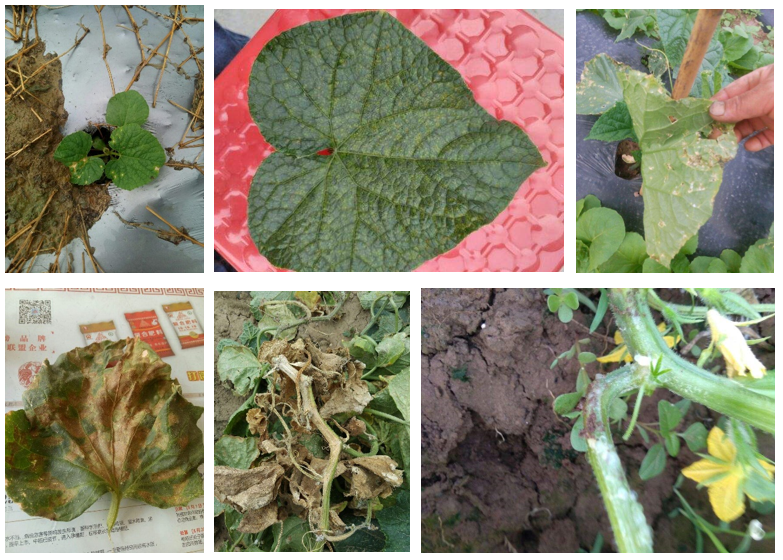
\includegraphics[width=0.75\textwidth]{figs_rev1/f1.png}
\caption{Cucumber complex background data set presentation}
\label{fig:f1}
\end{figure}

With the help of plant pathologists, these images are labeled and became the data set of this experiment. The data set consist of 2392 images, of which 80\% are used for the training set and 598 images (20\%), are used as the test set. As shown in the Figure\ref{fig:f2}, we propose a lightweight and fast MobileNetv3 network structure that can quickly and accurately complete the classification of seven kinds of cucumber leaf diseases. The seven pathologic conditions are downy mildew, powdery mildew, bacterial angular leaf spot, target leaf spot, gummy stem blight, fusarium wilt, and anthracnose. Therefore, the machine vision system for cucumber pathological diagnosis  proposed in this paper includes three steps: image acquisition, preprocessing and classification, and then the network model is optimized. This is shown in Figure\ref{fig:f2}.
\begin{figure}
\centering
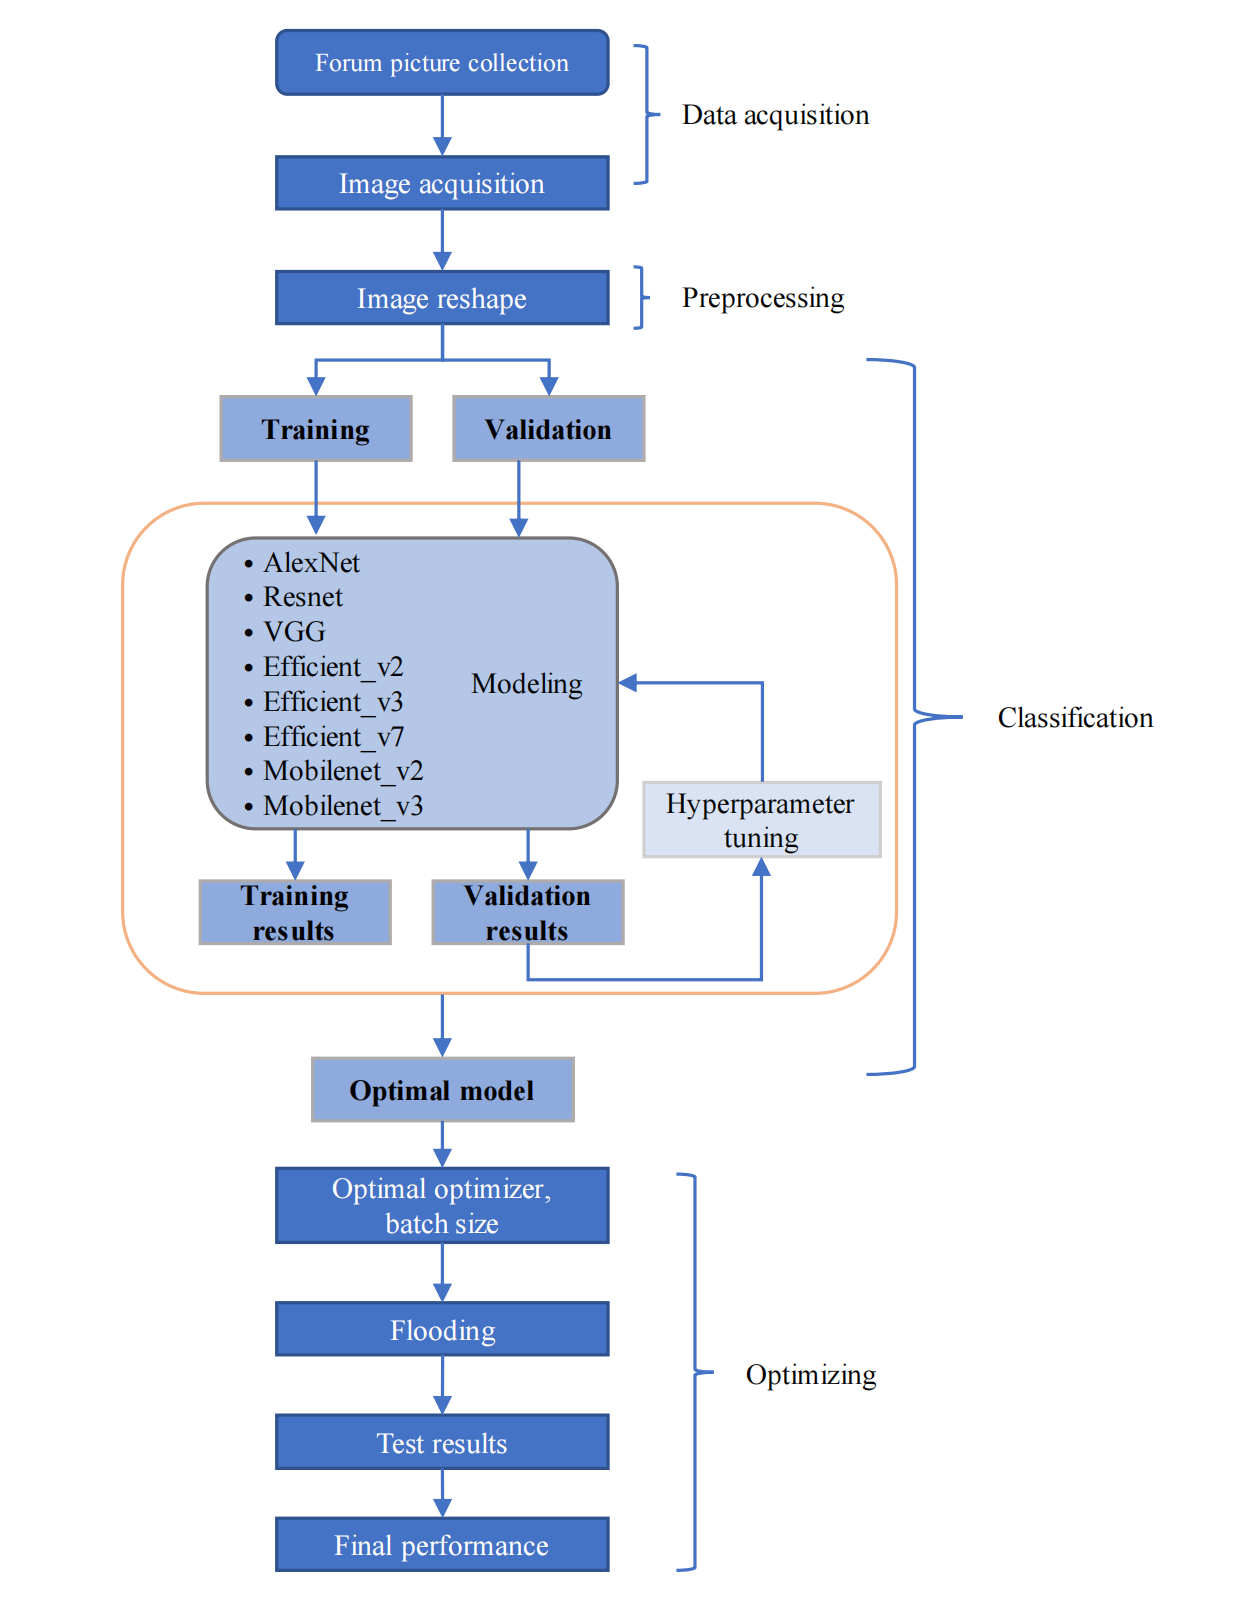
\includegraphics[width=0.75\textwidth]{figs_rev1/f2.png}
\caption{Article algorithm}
\label{fig:f2}
\end{figure}

\subsection{MobileNet v3}
MobileNetV3 is a lightweight network. MobileNetV3 uses a network architecture search (NAS) to search the global network structure by optimizing each network block, supplemented by the NetAdapt algorithm. This technique can efficiently determine an optimal model for a given hardware platform. In addition, MobileNetV3 uses the h-swish activation function to improve accuracy \citep{howard2019searching}

In contrast to other classification models, it operates a single convolution at each depth of the input image, rather than combining and flattening all the depths of the input image, which is achieved through depth-oriented separable convolution. This deep convolution divides the convolution process into two layers, one for filtering and the other for merging. This combination reduces the size of the model. MobileNetv3 consists of four 2D convolution layers, two (112x122) bottleneck layers, two (56×56) bottleneck layers, three (28×28) bottleneck layers, seven (14×14) bottleneck layers, and two (7×7) bottleneck layers, in which Swish and Relu are used as activation. Use a aggregaion layer (7x7) before two dense layers. Extrusion and excitation layers are also included to make it faster and lighter. This addition assigns unequal weights to channels when creating a map of output elements. Finally, a dense layer with 1024 units is applied to obtain the feature vector. The following Table\ref{tab:mbv3} shows the network structure of MobileNet v3 large. In the table, Input is the size of the input image, Operator is the convolution layer or the reciprocal residual structure, Exp size and Out are the number of convolution kernels in the first and last layer of the reciprocal residual structure, respectively, and SE is whether to use the SE module. NL is the activation function used in the first and second layers of the reciprocal residual structure, and S is the step length of the deep convolution layer of the reciprocal residual structure.
\begin{table}
\centering
\caption{$MobileNet\_v3\_large$ network structure}
\label{tab:mbv3}
\begin{tabular}{ccccccc}
\hline 
Input & Operator & Exp size & Out & SE & NL & S \\
\hline  
$224 \times 224 \times 3$  & conv2d &  $\times$  & 16 &  $\times$  & h-swish & 2 \\
 $112 \times 112 \times 16$  & bneck,  $3 \times 3$  & 16 & 16 &  $\times$  & relu & 1 \\
 $112 \times 112 \times 16$  & bneck,  $3 \times 3$  & 64 & 24 &  $\times$  & relu & 2 \\
 $56 \times 56 \times 24$  & bneck,  $3 \times 3$  & 72 & 24 &  $\times$  & relu & 1 \\
 $56 \times 56 \times 24$  & bneck,  $5 \times 5$  & 72 & 40 &  $\sqrt{ }$  & relu & 2 \\
 $28 \times 28 \times 40$  & bneck,  $5 \times 5$  & 120 & 40 &  $\sqrt{ }$  & relu & 1 \\
 $28 \times 28 \times 40$  & bneck,  $5 \times 5$  & 120 & 40 &  $\sqrt{ }$  & relu & 1 \\
 $28 \times 28 \times 40$  & bneck,  $3 \times 3$  & 240 & 80 &  $\times$  & h-swish & 2 \\
 $14 \times 14 \times 80$  & bneck,  $3 \times 3$  & 200 & 80 &  $\times$  & h-swish & 1 \\
 $14 \times 14 \times 80$  & bneck,  $3 \times 3$  & 184 & 80 &  $\times$  & h-swish & 1 \\
 $14 \times 14 \times 80$  & bneck,  $3 \times 3$  & 184 & 80 &  $\times$  & h-swish & 1 \\
 $14 \times 14 \times 80$  & bneck,  $3 \times 3$  & 480 & 112 &  $\times$  & h-swish & 1 \\
 $14 \times 14 \times 112$  & bneck,  $3 \times 3$  & 672 & 112 &  $\sqrt{ }$  & h-swish & 1 \\
 $14 \times 14 \times 112$  & bneck,  $5 \times 5$  & 672 & 160 &  $\sqrt{ }$ & h-swish & 2 \\
 $7 \times 7 \times 160$  & bneck,  $5 \times 5$  & 960 & 160 &  $\sqrt{ }$  & h-swish & 1 \\
 $7 \times 7 \times 160$  & bneck,  $5 \times 5$  & 960 & 160 &  $\sqrt{ }$  & h-swish & 1 \\
$7 \times 7 \times 160$  & conv2d,  $1 \times 1$  &  $\times$  & 960 &  $\times$  & h-swish & 1 \\
 $7 \times 7 \times 960$  & pool,  $7 \times 7$  &  $\times$  &  $\times$  &  $\times$  &  $\times$  & 1 \\
 $1 \times 1 \times 960$  & conv2d  $1 \times 1$, $\mathrm{NBN}$  &  $\times$  & 1280 &  $\times$  & h-swish & 1 \\
 $1 \times 1 \times 1280$  & conv2d  $1 \times 1$, $\mathrm{NBN}$  &  $\times$  &  $\mathrm{k}$  &  $\times$  &  $\times$  & 1 \\
\hline
\end{tabular}
\end{table}

\subsection{Flooding}
In this paper, the superiority of the network model is judged mainly by the loss size. Firstly, we introduce the generation mathod of loss function. This paper's experiment's loss function adopts the cross entropy loss function to classify the pathology of cucumber leaves into seven categories: $C=7$ and batch capacity $N=12$. The calculation formula of the loss function is as follows.\ref{eq:eq1}:
\begin{equation}
\label{eq:eq1}
\ell(p, q)=L=\left\{l_{1}, \ldots, l_{N}\right\}^{\top}, \quad l_{m}=-\sum_{c=1}^{C} w_{c} \log \frac{\exp \left(x_{m, c}\right)}{\sum_{i=1}^{C} \exp \left(x_{m, i}\right)} y_{m, c}
\end{equation}

Where x is the input,y is the target, w is the weight, and l is the loss function value. 

The loss value of each data sample is calculated through the cross-entropy loss function. Then the total loss function of an epoch is added and calculated according to the batch size to obtain the loss value of the image in our chapter 4 experiment. That is,\ref{eq:eq2}:
\begin{equation}
\label{eq:eq2}
\ell(p,q)=\sum_{m=1}^{N} l_{m}
\end{equation}

In this paper, the size of the loss function is taken as the benchmark for the superiority of the network model. In the follow-up experiments, we will find that the network model we used has an over-fitting phenomenon. A loss evaluation 192
strategy needs to be replaced. After reaching a certain threshold, we will  not take the simple loss decline as the training orientation. This will make the loss on the test set shows a relatively flat trend, and then the rising speed of the loss on the test set will be reduced, and even a secondary decline may occur. Finally, the accuracy is further improved to a certain extent. We need a way to solve this problem, and the flooding method came into being. \citep{ishida2020we}

% 本段为需要降重段
Consider input variable  $\boldsymbol{p} \in \mathbb{J}^{d}$  and output variable  $q \in   [C]:=\{1, \ldots, C\}$ , where  C  is the number of classes. They follow an unknown joint probability distribution with density  $p(\boldsymbol{p}, q)$ . We denote the score function by  $\boldsymbol{f}: \mathbb{J}^{d} \rightarrow   \mathbb{J}^{C}$ . For any test data point  $p_{0}$ , our prediction of the output label will be given by  $\widehat{q}_{0}:=\arg \max _{z \in[C]} f_{z}\left(p_{0}\right)$ , where  $f_{z}(\cdot)$  is the  $z$ -th element of  $f(\cdot)$ , and in case of a tie, arg max returns the largest argument. Let  $\ell: \mathbb{J}^{C} \times[C] \rightarrow \mathbb{J}$  denote a loss function.  $\ell$  can be the zero-one loss, where  $w:=\left(w_{1}, \ldots, w_{C}\right)^{\top} \in \mathbb{J}^{C}$ , or a surrogate loss such as the softmax cross-entropy loss,\ref{eq:eq3}:
\begin{equation}
\label{eq:eq3}
\ell_{\mathrm{CE}}\left(\boldsymbol{w}, z^{\prime}\right):=-\log \frac{\exp \left(w_{z^{\prime}}\right)}{\sum_{z \in[C]} \exp \left(w_{z}\right)} .
\end{equation}
For a surrogate loss  $\ell$ , we denote the classification risk.
The goal of multi-class classification is to learn  $f$  that minimizes the classification error  $J_{01}(f)$ . In optimization, we consider the minimization of the risk with a almost surely differentiable surrogate loss  $J(\boldsymbol{f})$  instead to make the problem more tractable. Furthermore, since  $p(p, q)$  is usually unknown and there is no way to exactly evaluate  $J(\boldsymbol{f})$ , we minimize its empirical version calculated from the training data instead\ref{eq:eq4}:
\begin{equation}
\label{eq:eq4}
\widehat{J}(\boldsymbol{f}):=\frac{1}{m} \sum_{i=1}^{m} \ell\left(\boldsymbol{f}\left(\boldsymbol{p}_{i}\right), q_{i}\right)
\end{equation}
where  $\left\{\left(p_{i}, q_{i}\right)\right\}_{i=1}^{m}$  are i.i.d. sampled from  $p(p, q)$ . We call  $\widehat{J}$  the empirical risk.

$\mathbf{Definition 1.}$ The flooded empirical risk is defined  as \ref{eq:eq4} 
\begin{equation}
\widetilde{J}(\boldsymbol{f})=|\widehat{J}(\boldsymbol{f})-b|+b
\end{equation}
Note that when  $b=0$ , then  $\widetilde{J}(\boldsymbol{f})=\widehat{J}(f)$ . The gradient of  $\widetilde{J}(f)$  w.r.t. model parameters will point to the same direction as that of  $\widehat{J}(\boldsymbol{f})$  when  $\widehat{J}(\boldsymbol{f})>b$  but in the opposite direction when  $\widehat{J}(\boldsymbol{f})<b$ . This means that when the learning objective is above the flood level, we perform gradient descent as usual (gravity zone), but when the learning objective is below the flood level, we perform gradient ascent instead (buoyancy zone).Pushing the parameters towards a more stable region keeps the convergence of the loss function near a threshold value, which improves the generalization performance and better resists perturbations.
%

\section{Results and Discussion}
In this experiment, we first preprocess the image, and the PyTorch framework is used to scale the image to $448\times448$ for data standardization. In this paper, the Mobilenet v3 network model is selected as well as optimizer ASGD, the learning rate is set to $0.001$, the L1 regularity coefficients are all $0.01$, the batch size is $12$, and $300$ rounds of iterative training are conducted on the training set and the test set respectively. In order to prevent over-fitting phenomenon in the experiment, we also apply the algorithm of Dropout to randomly inactivate the neural nodes in the network before network training, reduce the interdependence between neurons, so as to ensure the extraction of important features that are independent of each other and improve the generalization ability of the model. As shown in the figure, it can be clearly seen that neurons randomly deactivate seven neural nodes in the network.
\begin{figure}
\centering
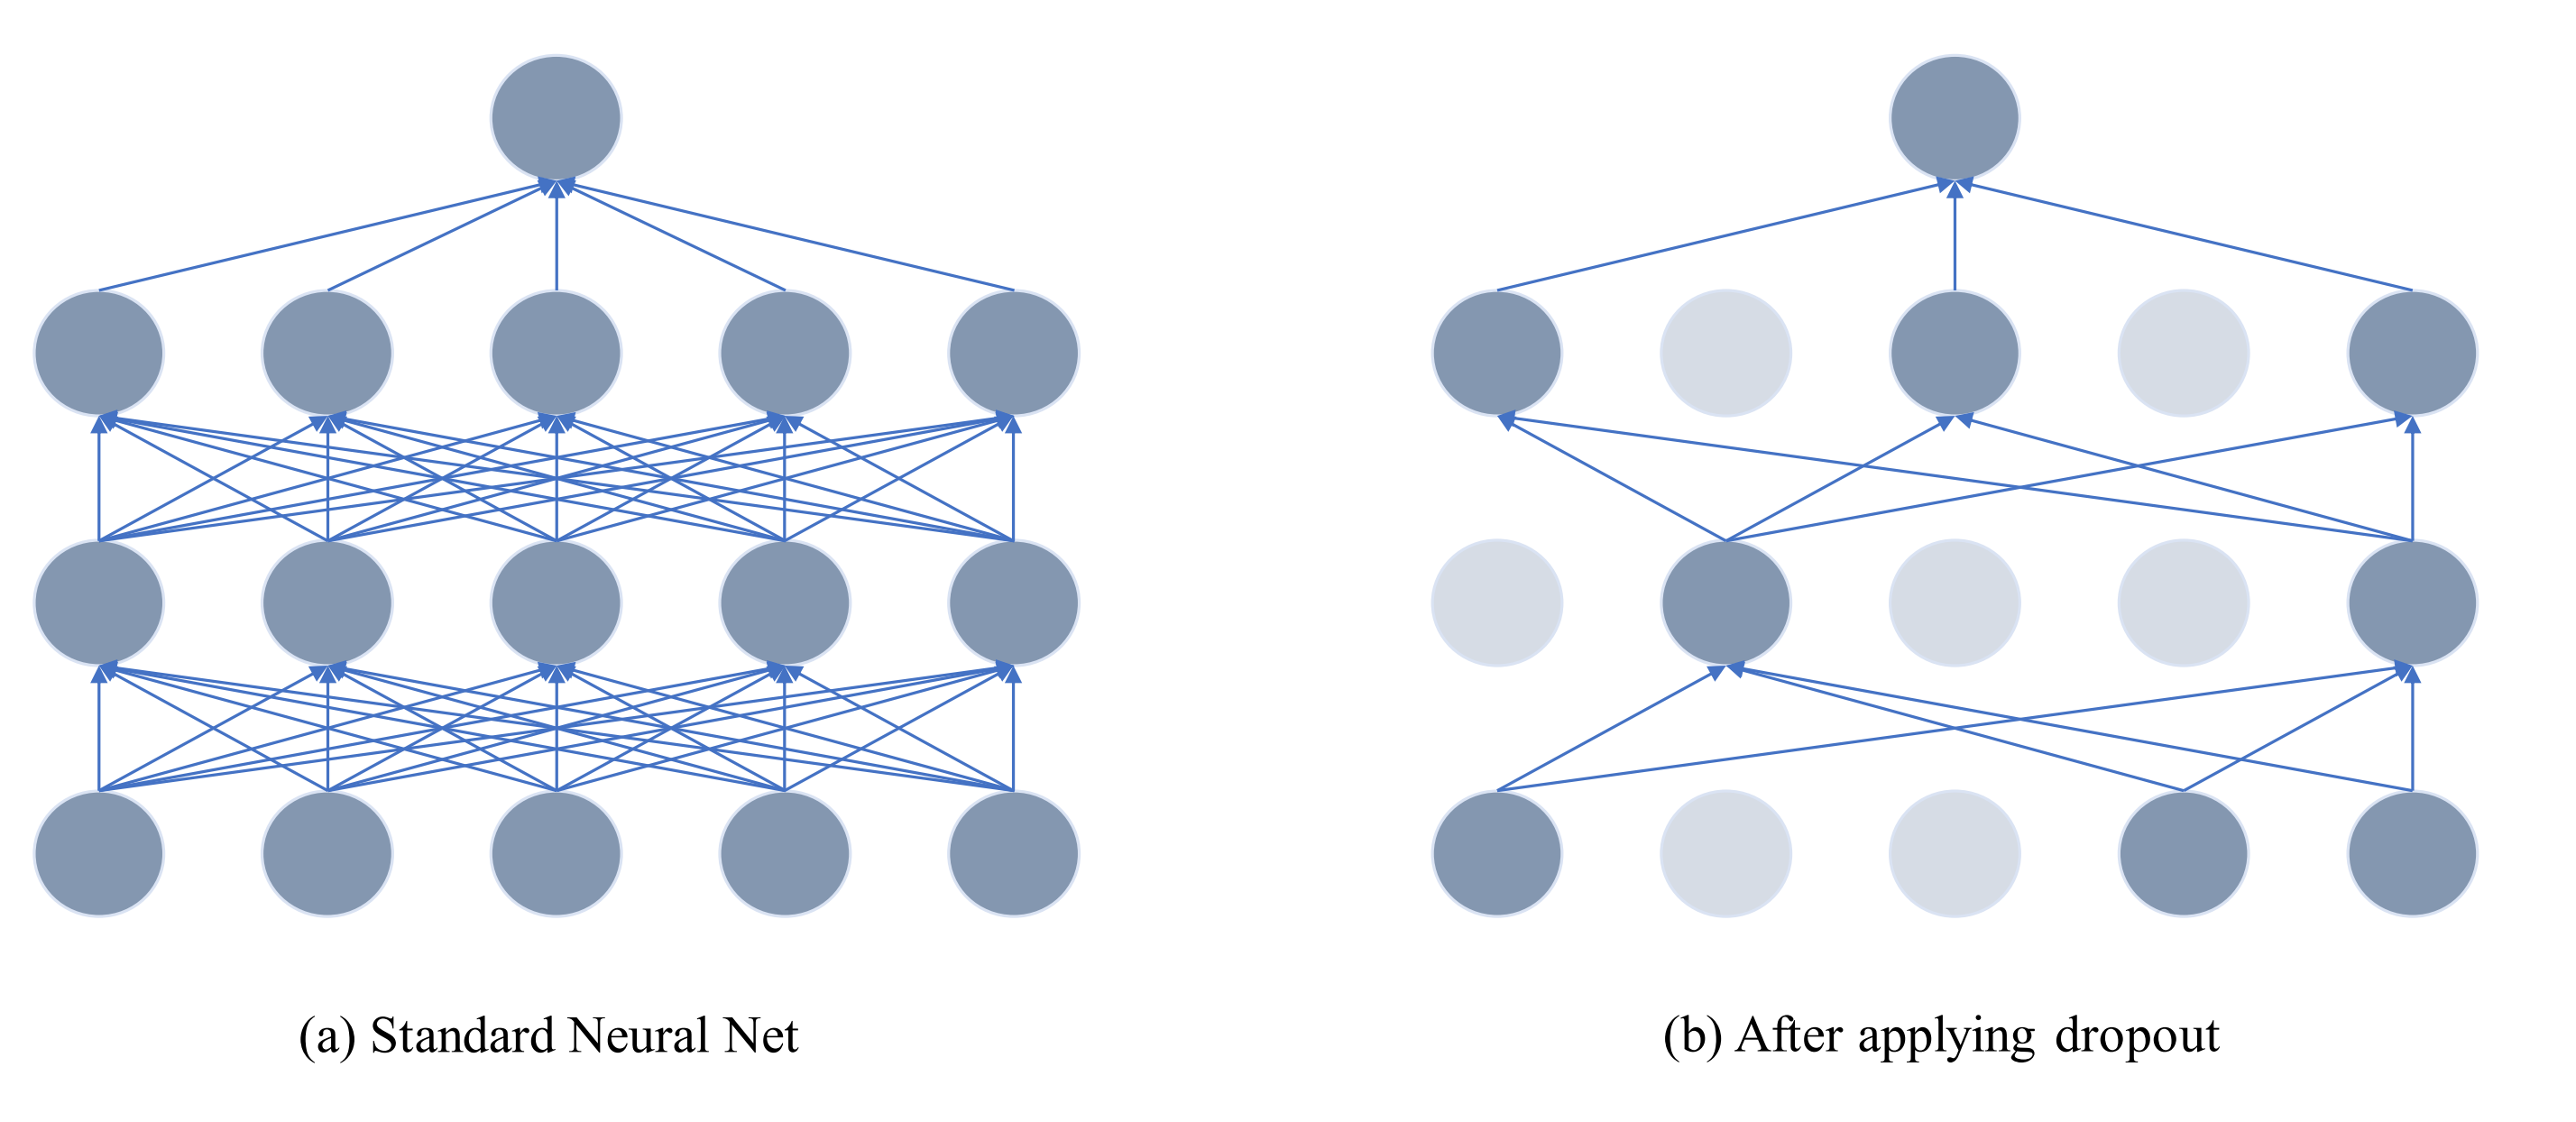
\includegraphics[width=0.75\textwidth]{figs_rev1/f3.png}
\caption{ A comparison of the neural network before and after using dropout}
\label{fig:f3}
\end{figure}

\subsection{Contrast test}
On the same cucumber pathological leaf image data set, we select seven current mainstream network models and MobileNet v3 network for comparative test. and accurately reflect the advantages of MobileNet v3 network from the experimental data. 

In this paper, Alexnet, Resnet, VGG, Efficientnet v2, Efficientnet v3, Efficientnet v7, Mobilenet v2, and Mobilenet v3 leaf pathological recognition models are trained, and image training set and test set are used to test and compare them. This way, the network model performance's superiority is tested and further optimized. The figure\ref{fig:f4} shows the experimental results, in which vg19 represents the VGG  model, alex represents Alexnet model, re50 represents Resnet model, mob3 represents Mobilenet v3 model, mob2 represents mobilenet v2 model, eff7 represents the efficient v7 model, eff3 represents the efficient v3 model, and eff2 represents the efficient v2 model. 
\begin{figure}
\centering
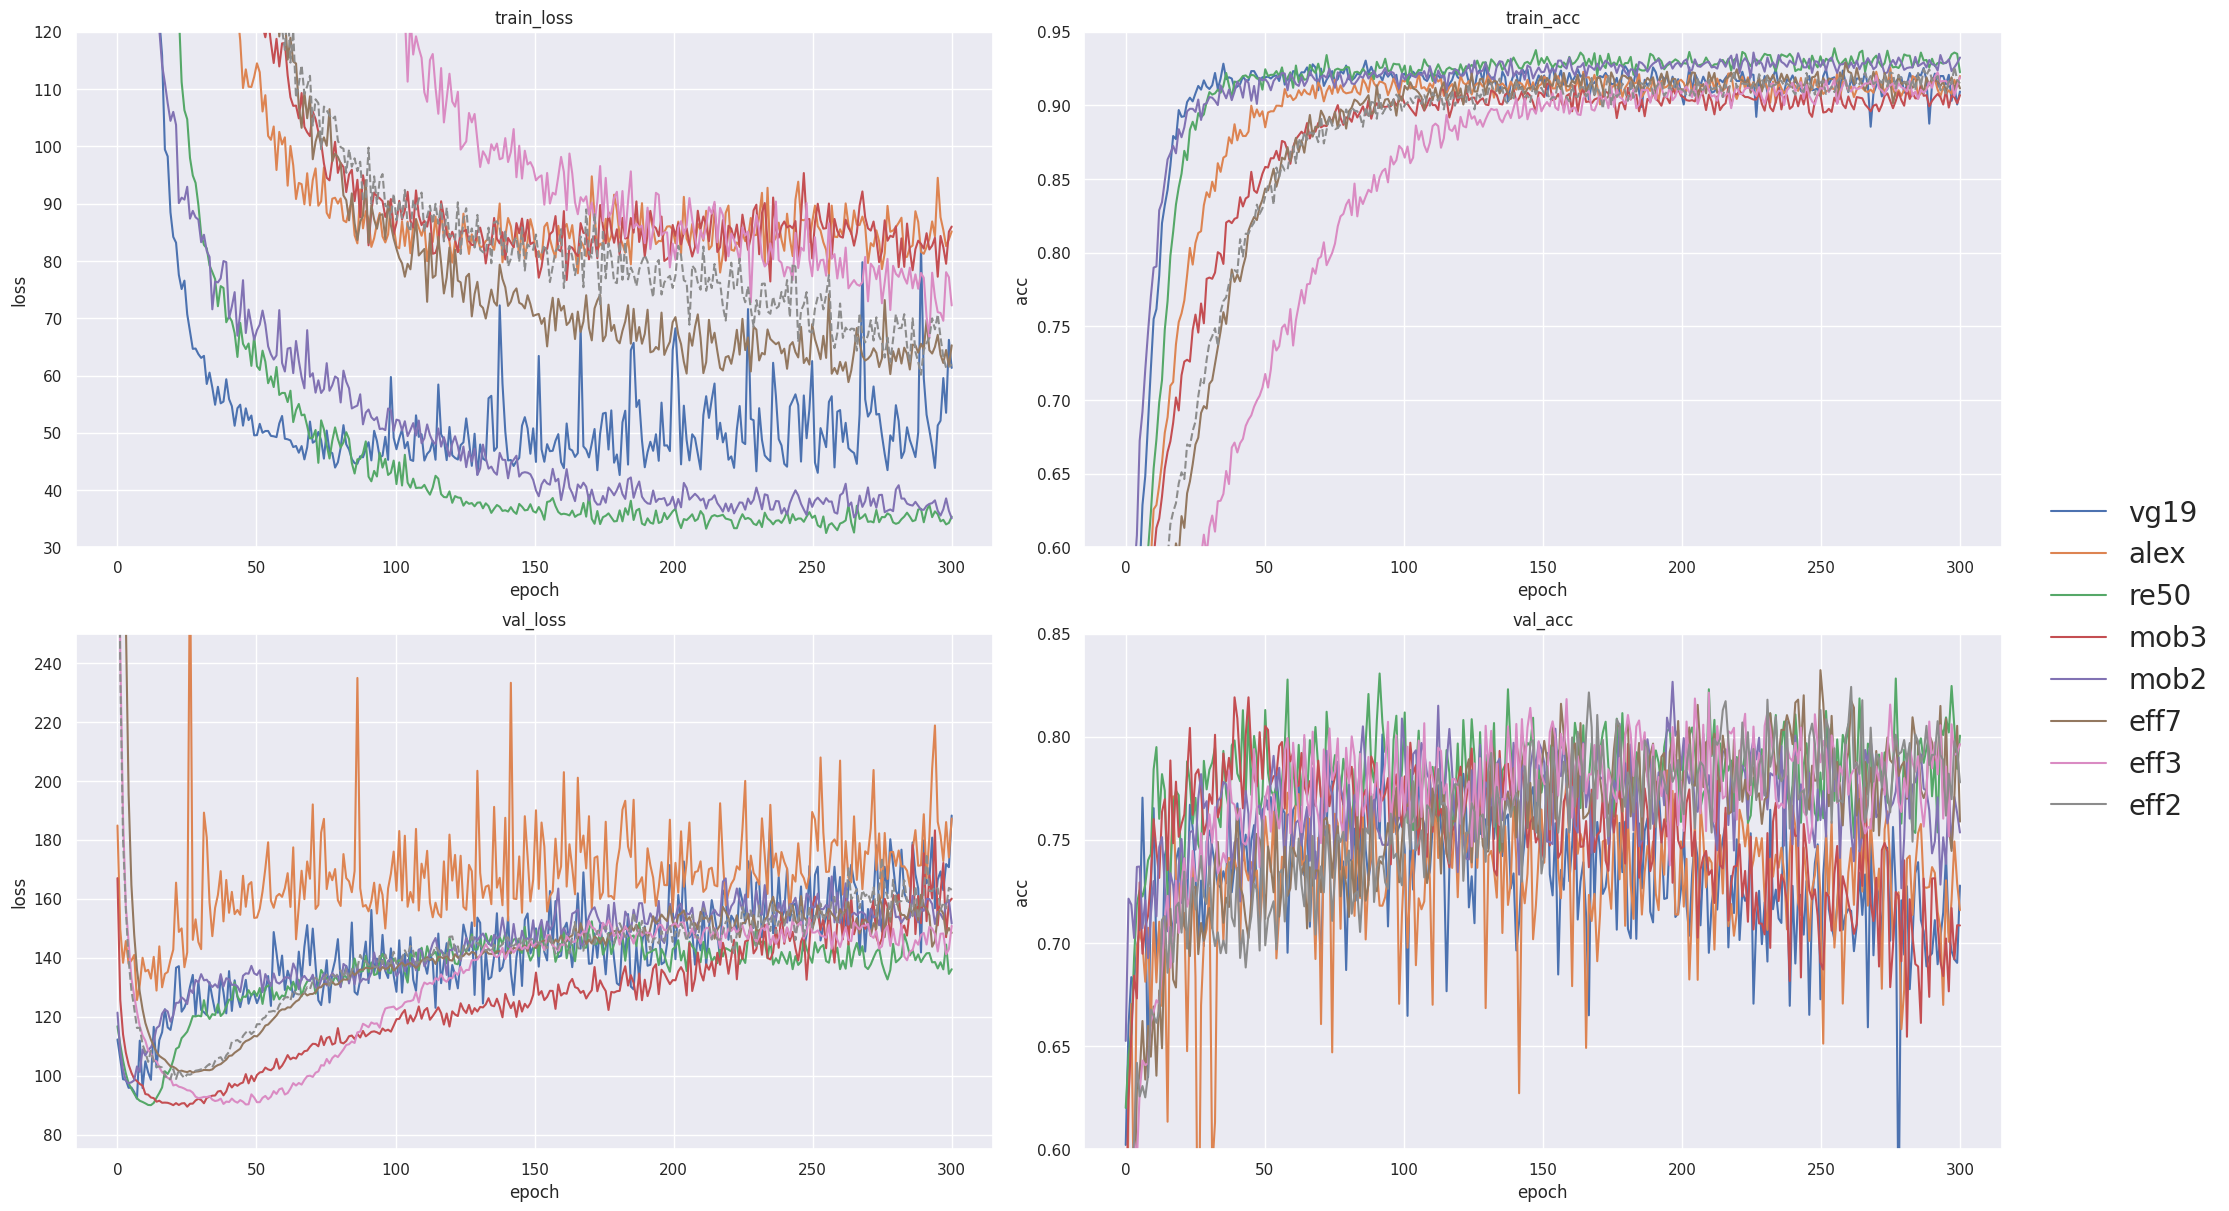
\includegraphics[width=0.75\textwidth]{figs_rev1/f4.png}
\caption{Comparison Experiment between mobilenet v3 and Mainstream Image Classification Algorithms}
\label{fig:f4}
\end{figure}

The loss function and accuracy of the training set of Alexnet model converge well. When epoch=100, they begin to converge and gradually become stable. However, the effect on the test set is not good, the fluctuation of loss and accuracy is large, and the convergence effect is not good. Compared with other models, its loss in the test set is highest, its accuracy is lowest, and its performance is poor. 

The training set of the VGG model converges quickly, and the loss image of the data set begins to converge in the 70th round of iteration. The accuracy image of the training set and the test set converge faster and it has converged in about 30 iteration rounds. However, the degree of fitting in the test set is not high, and the test set loss and accuracy image of the VGG model show no convergence trend. The average accuracy has not reached 70\%. 

The training set of Resnet begins to converge when the number of training rounds is around 40, and the convergence speed is very fast. When testing the test set, we found that the convergence fitting degree is considerably high, and the maximum accuracy is up to 81.4\%. However, the fluctuation range of loss and accuracy of the test set is numerically larger than that of Alexnet network model, and the loss function also appears to be an over-fitting phenomenon. 

The results of Efficientnet v2 and Efficientnet v7 models are basically the same. The loss and accuracy of the test set tend to converge, and the fitting degree is also higher compared with the training set. However, the degree of over-fitting of the loss image of the test set is too high and fluctuates wildly. 

The Efficientnet v3 model, where the precision image of the test set begins to converge around the 150th iteration round, is the slowest of all models. The test set of Efficientnet v3 shows a convergence effect, but a severe over-fitting phenomenon occurs, and the fluctuation is the largest from the experimental results. 

In the MobileNet v2 model, the training set starts to converge from the 30th iteration, and the loss finally keeps approaching 0, and the accuracy also keeps increasing with the training rounds. The result trend of the test set also roughly fits the training set, but there is an over-fitting phenomenon with low generalization and large fluctuation.

Considering the fitting effect of each model test set comprehensively, the test set result trend of Mobilenet v3 network is consistent with the training set trend, and its maximum accuracy is relatively the highest, reaching 81.3\% and above. Moreover, Mobilenet v3 converges 66\% faster than Resnet network and much faster than any other network due to its lightweight framework. Therefore, Mobilenet v3 network is finnaly chosen for the next optimization experiment.

\subsection{The choice of optimizer}
After selecting Mobilenet v3 as the final experimental network, this paper will optimize it. The first step is the selection of the optimizer. Optimizer is used to update and calculate network parameters that affect model training and model output, so that network can reach the optimal value, thereby minimizing (or maximizing) the loss function. Choosing an appropriate optimizer can make our network model reach convergence faster and achieve better accuracy. On the same cucumber pathological leaf image data set, Mobilenet v3 network is selected in this paper, and the learning rate is set to 0.001. The regularity coefficients of L1 and L2 are both 0.01, and 300 rounds of iterative training are conducted on the training set and test set respectively. In this paper, ASGD, SGD, RMSprop, RAdam, NAdam, AdamW, Adamax, Adadelta, and Agagrad are selected for comparison. Loss functions and accuracy images of the training set and test set are obtained, as shown in the figure \ref{fig:f5}.
\begin{figure}
\centering
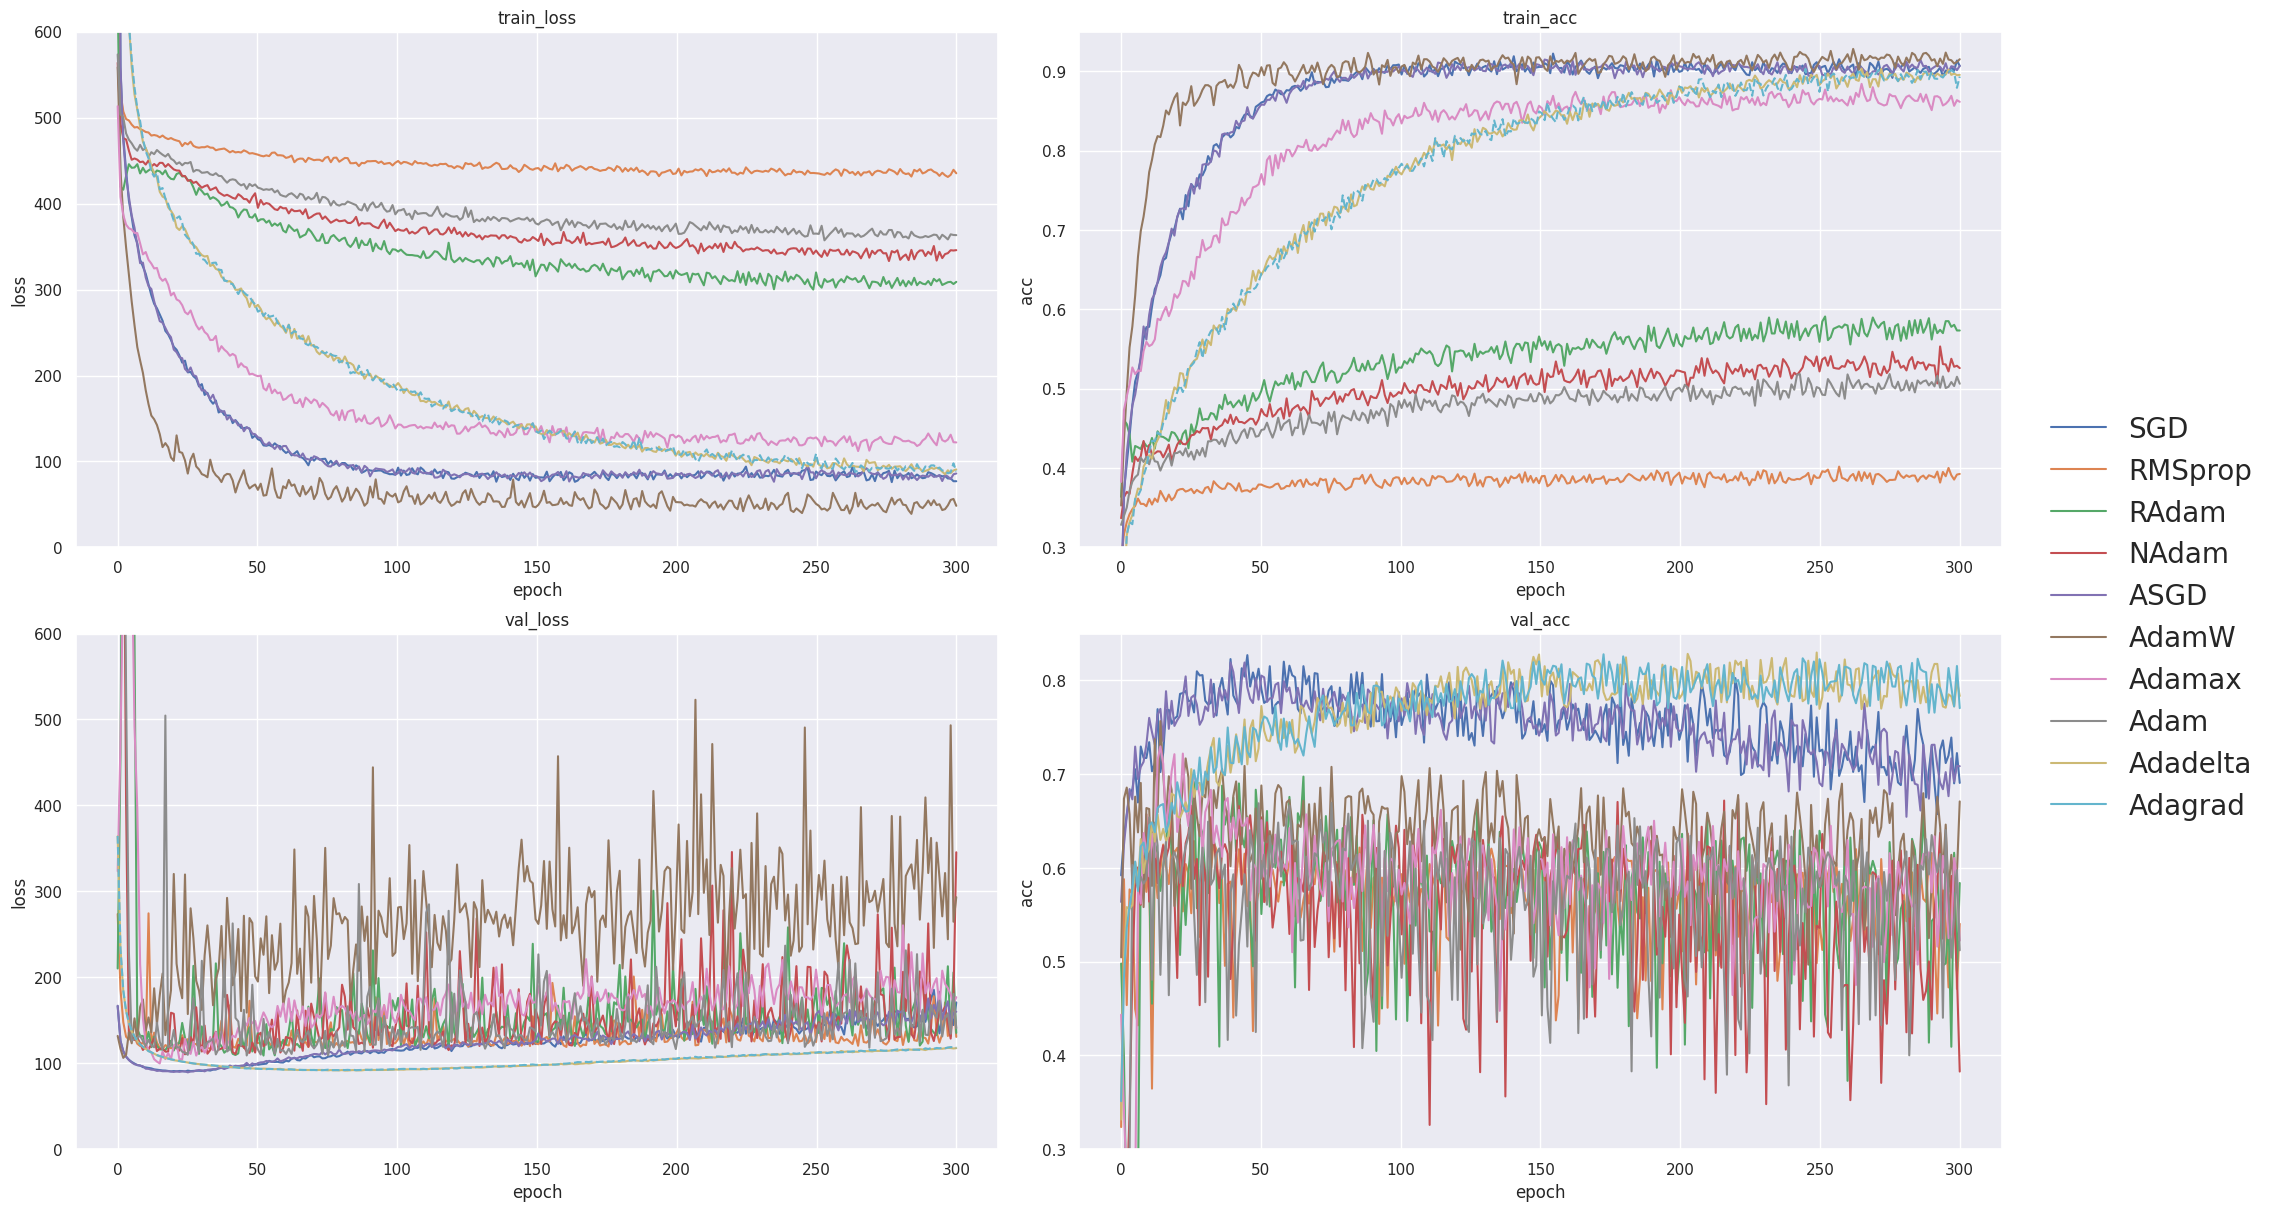
\includegraphics[width=0.75\textwidth]{figs_rev1/f5.png}
\caption{Comparison Experiment between ASGD and Mainstream Optimizer Experiment}
\label{fig:f5}
\end{figure}

As shown in the figure \ref{fig:f5}, although the four optimizers, RAdam, NAdam, Adam, and RMSprop, all have a convergence trend at last, their loss value in the training set are very high, and their highest accuracy is not more than 60\%. Compared with other optimizers, the effect of those four optimizers is poor. RAdam, NAdam, Adam, and RMSprop are unsuitable for this paper's network model. 

AdamW optimizer performs well in the training set. The convergence rate of the loss function and accuracy image is the fastest compared with other optimizers. However, its performance in the test set could be better. The loss function and accuracy image have large fluctuations, and its maximum accuracy is at most 70\%. 

Adamax optimizer begins to converge after 100 iteration rounds of the training set, and its loss function image value in the test set is higher than that of the ten optimizers, its accuracy is low, with an average accuracy of less than 65\%. 

The data set images of Adadelta and Adagrad optimizers almost coincide. Both the training set and the test set converge. The loss value gradually decreases with the increase in the number of iterations, which is the lowest among the ten optimizers. The accuracy also increases with the number of iterations, reaching a high accuracy of 83\%. However, its convergence speed is very slow. The training set begins to converge in the 250th iteration round, and the test set begins to converge in the 150th iteration round, which takes the longest time. 

The data set images of the two optimizers, ASGD and SGD, almost coincide, converge in both the training set and the test set, and the convergence is faster. The training set begins to converge in the 80th iteration round, and the test set begins to converge in the 20th iteration. And the peak value of test set accuracy is the highest, up to 81.4\%. Numerically, the ASGD has less fluctuation than the SGD optimizer. 

Therefore, after comparing convergence speed, fitting degree, accuracy, loss function size, and other aspects, ASGD has a higher peak value, faster convergence, and minor fluctuation. In this article, the ASGD is chosen as the final optimizer.

\subsection{The choice of batch size}
In this comparison experiment, Mobilenet v3 network model is selected, the optimizer is ASGD, the learning rate is set to 0.001, the regularity coefficients of L1 and L2 are both 0.01, and 300 rounds of iterative training are conducted on the training set and test set respectively. Batch size is selected as 4, 8, 12, 16, 20, 24, 28, and 32. The images and data results are obtained as shown in the figure below. \ref{fig:f6}
\begin{figure}
\centering
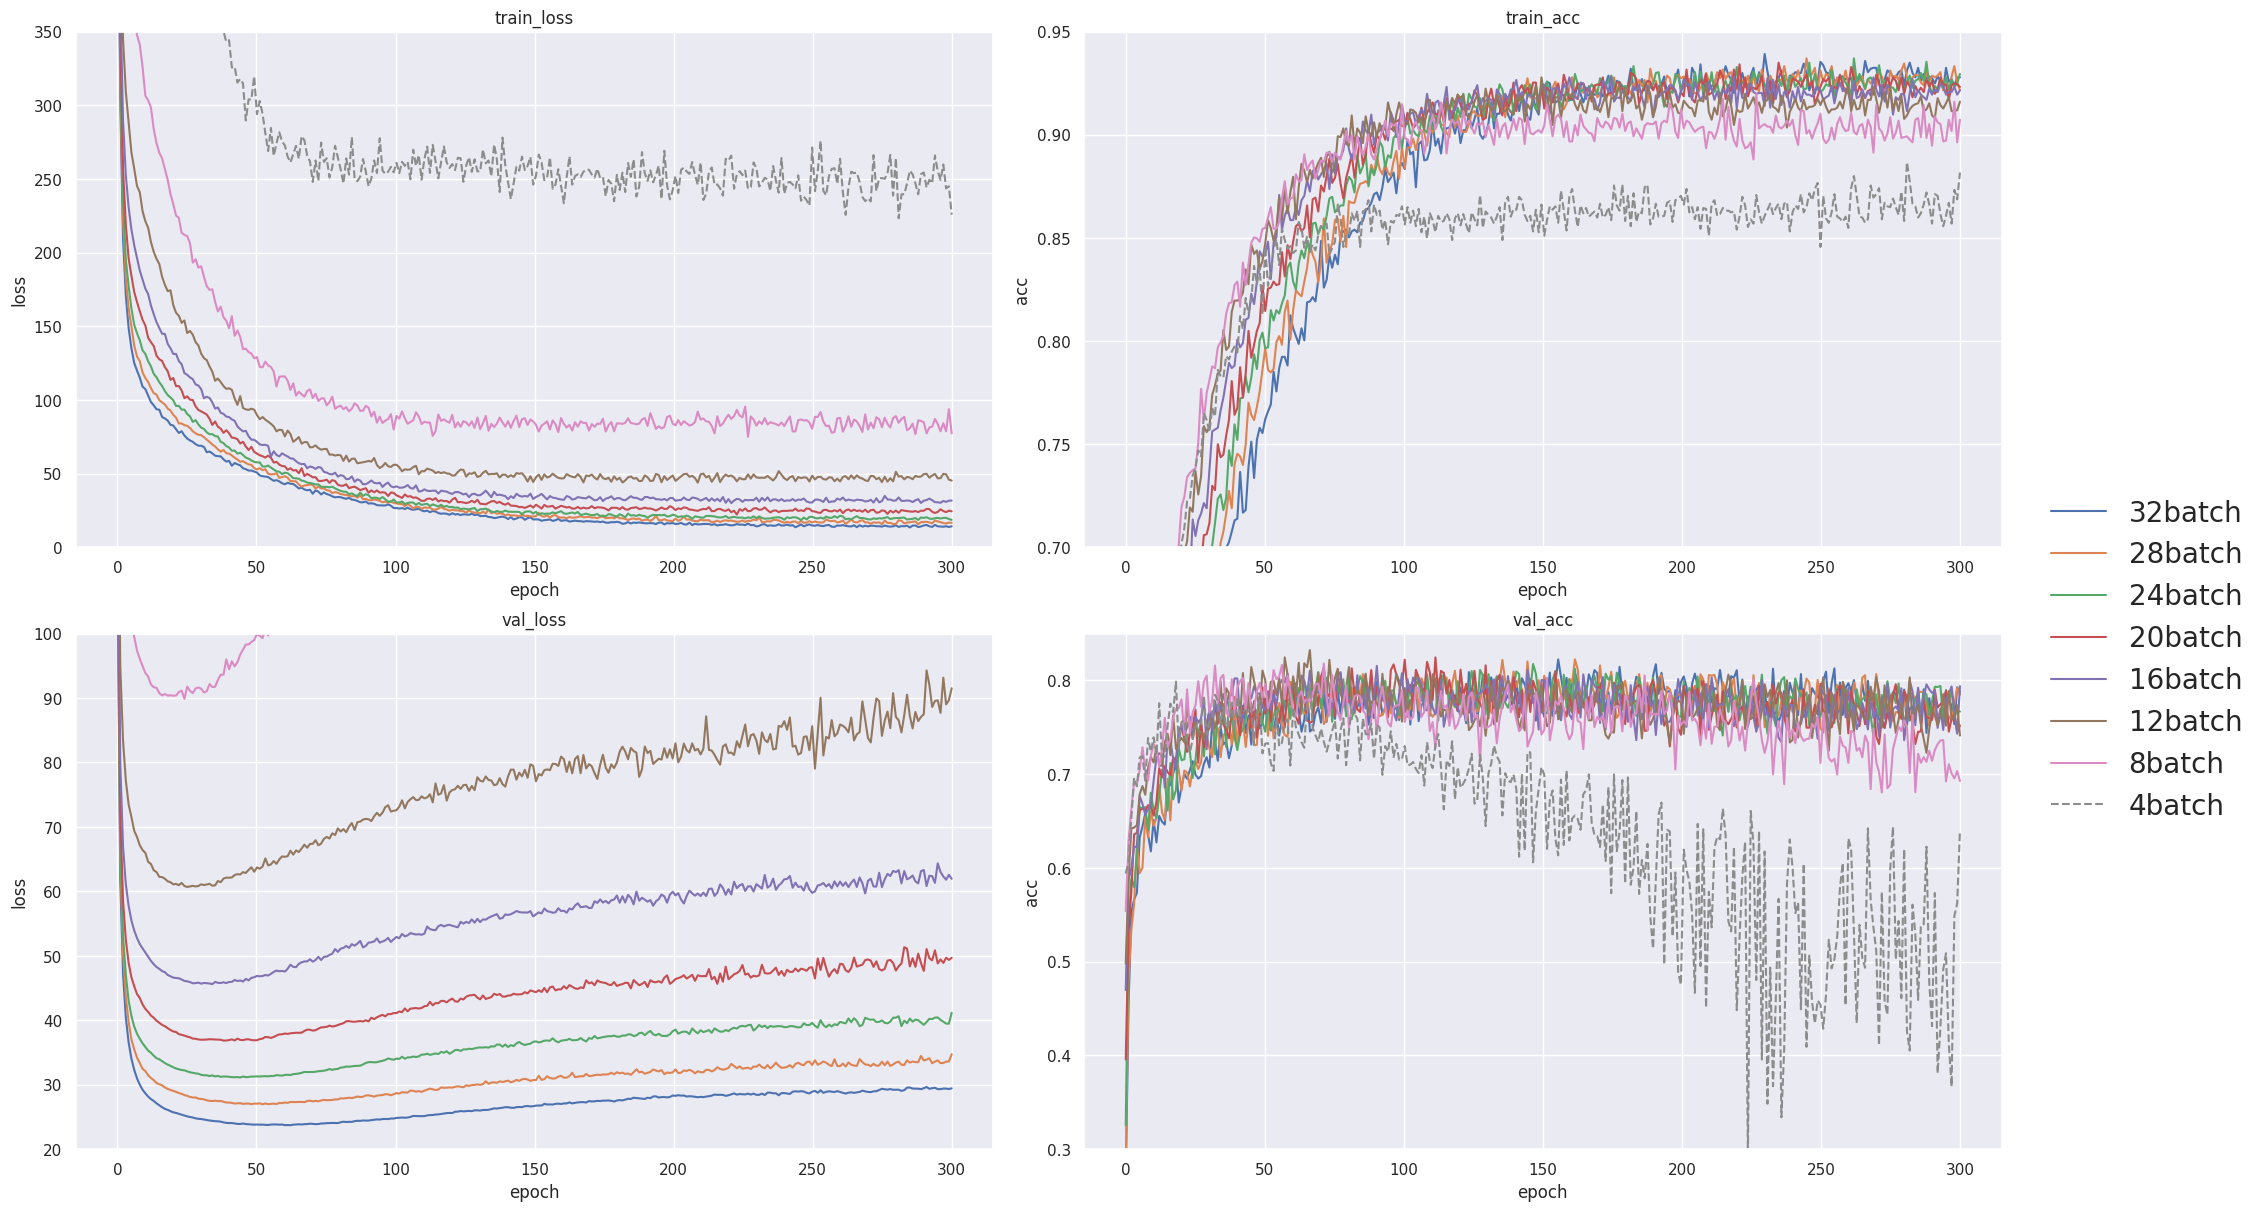
\includegraphics[width=0.75\textwidth]{figs_rev1/f6.png}
\caption{Comparative Experiments with Different batch Sizes}
\label{fig:f6}
\end{figure}

%4.3 batch_size的table
\begin{table}
\centering
\caption{Use effect of different batch sizes}
\label{tab:mbv5}
\begin{tabular}{ccccccc}
\hline 
batch\_size & max\_acc(\%) & mean\_acc(\%) & sstd\_acc(\%) & max\_loss & mean\_loss & std\_loss \\
\hline  
4   & 79.870 &  64.197  & 10.916 &  1367.639  & 367.173 & 181.912 \\
 8   & 81.794  & 75.492 & 3.227 &  178.613  & 125.196 & 20.972 \\
 12   & 82.115   & 76.568 & 2.962 &  135.261  & 76.619 & 9.009 \\
 16  & 81.542   & 76.848 & 3.556 &  123.976  & 55.940 & 6.853 \\
 20  &  82.451  & 76.626 & 4.069 &  118.699  & 44.232 & 6.210 \\
 24  & 81.751  & 76.854 & 4.498 &  117.166  & 36.638 & 5.916 \\
 28  & 82.245  & 76.527 & 5.140 &  113.502  & 31.251 & 5.801 \\
 32  & 82.230  & 76.486 & 5.303 &  112.958  & 27.393 & 5.897 \\
\hline
\end{tabular}
\end{table}

Batch $size=4$, as the batch size value is too small, the gradient of each layer has high randomness and takes much time. The resulting image also fluctuates, and the final precision effect is considerably poor, resulting in an under-fitting phenomenon. The convergence effect is not good enough. 

It can be seen from the figure\ref{fig:f6} that the convergence speed increases with the increase of batch size. According to the numerical results in \ref{tab:mbv5}, with the increase of batch size, the maximum loss function, average loss function, and the standard deviation of the loss function, namely the volatility, of the test set gradually decrease. However, after batch $size=12$, each loss value changes little with the increase in batch size. In addition, the maximum accuracy after convergence increases weakly and sometimes even regresses. Moreover, after batch $size=12$, the standard deviation of the accuracy of the test set began to rise continuously, indicating that the model's generalization ability declined. Before batch $size=12$, the test set's accuracy increases while the loss fluctuation decreases. When batch $size=12$, the standard deviation of loss is minimum, and the anti-aliasing effect is best. At the same time, the accuracy of the test set increased to 82.1\%. 

The experiment in this paper is carried out under a blurred background image, so we need as much generalization ability as possible. Moreover, the model proposed in this paper should apply to mobile terminal devices, should be as lightweight as possible, and need to select the smallest batch size value possible. Therefore, from the perspective of background requirements and image data analysis, batch $size=12$ is selected as the optimal experimental parameter in this paper.

\subsection{Flooding}
In Chapter 3, we introduce the basic principle and used a flooding mode. that is, by changing the loss function and adding a threshold, the loss eventually fluctuated around the threshold. Flooding allows us to directly select the level of training loss, which is difficult to achieve with other regularizers. There is an over-fitting phenomenon in the loss result in images of the Mobilenet v3 experiment mentioned above. In this section, flooding is used to realize the secondary decrease of data set loss and prevent over-fitting. 

In this experiment, the optimizer uses ASGD, the learning rate is 0.001, the regularization coefficients of L1 and L2 are 0.01, and 300 iteration experiments were conducted. The loss threshold is set with 15 different values for comparative analysis of images and data.
\begin{figure}
\centering
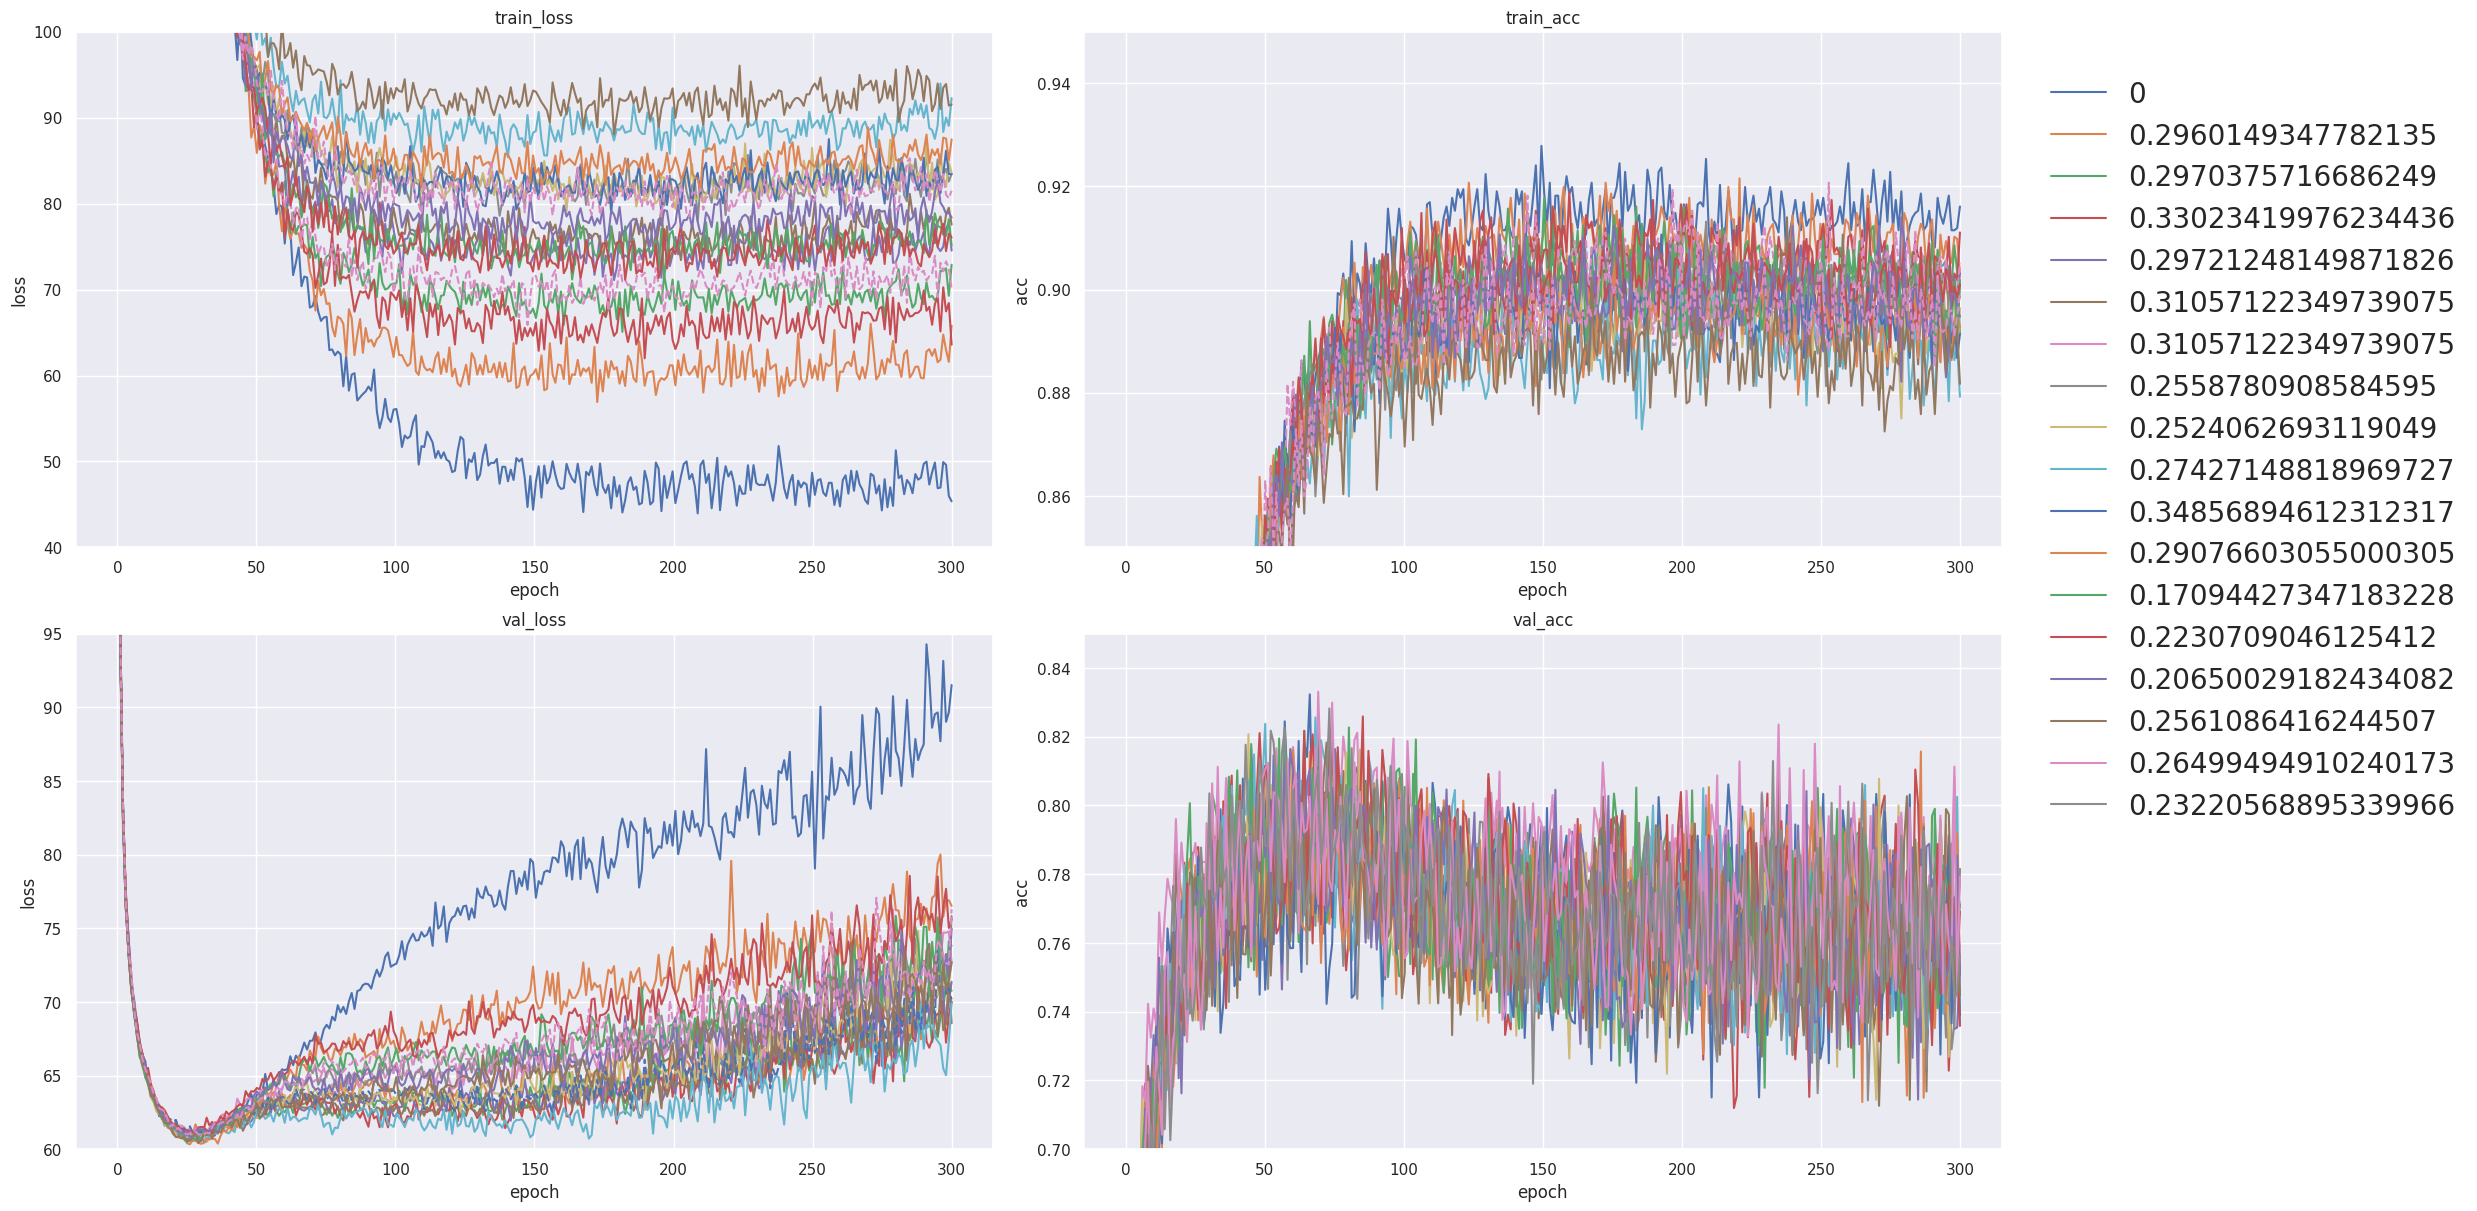
\includegraphics[width=0.75\textwidth]{figs_rev1/f7.png}
\caption{Comparative Experiment on Different Values of Parameter b After Using flooding}
\label{fig:f7}
\end{figure}

As seen from the image,\ref{fig:f7} after flooding is added, the over-fitting rising trend of the loss function image of the test set is effectively suppressed. When $b=0.310$, $0.348$, and $0.290$, the flooding not only resulted in good inhibition but also resulted in secondary descending, which solved the over-fitting problem.

%4.4 flooding的table
\begin{table}
\centering
\caption{Use effect after different values of parameter b in flooding}
\label{tab:mbv4}
\begin{tabular}{ccccccc}
\hline 
b & max\_acc(\%) & mean\_acc(\%) & sstd\_acc(\%) & max\_loss & mean\_loss & std\_loss \\
\hline  
0.349   & 81.644 &  76.025  & 2.980 &  139.207  & 63.706 & 5.395 \\
 0.291   & 81.608  & 76.508 & 3.076 &  136.610  & 65.388 & 5.288 \\
 0.252   & 82.068   & 76.344 & 3.080 &  138.879  & 67.156 & 5.405 \\
 0.311  & 83.308   & 78.263 & 2.658 &  135.187  & 64.881 & 5.256 \\
 0.297  &  81.641  & 76.315 & 2.980 &  139.065  & 65.060 & 5.400 \\
 0.330  & 80.890  & 76.395 & 3.248 & 138.475   & 64.670 & 5.387 \\
 0.297  & 81.375  & 76.458 &    2.953  & 138.858 & 64.929&5.319 \\
 0.296  & 81.568  & 76.385 & 3.146 &  137.580  & 65.504 & 5.320 \\
 0.274  & 82.557 &  76.497  & 3.249 &  136.909  & 65.820 & 5.494 \\
 0.171   & 82.271  & 76.717 & 3.136 &  136.269  & 69.950 & 6.173 \\
 0.232   & 82.820   & 76.610 & 3.306 &  136.021  & 67.736 & 5.490 \\
 0.265  & 81.786   & 76.702 & 3.238 &  134.727  & 66.250 & 5.396 \\
 0.256  &  81.828  & 76.217 & 3.118 &  138.510  & 66.854 & 5.473 \\
 0.207  & 81.634  & 76.496 & 3.263 &  137.237  & 69.357 & 5.813 \\
 0.223  & 82.588  & 76.782 & 3.382 &  136.995  & 67.819 & 5.571 \\
\hline
\end{tabular}
\end{table}

According to a series of comparisons of the table data, after adding flooding to \ref{tab:mbv4}, the mean test set accuracy increased by 0.2\%, and the maximum test set accuracy increased by 0.5\%. The final goal of this paper is to select the test set with the highest accuracy to achieve the best pathological recognition effect of the cucumber leaf image. The final selection threshold is 0.310, at which time the over-fitting of the loss function is well suppressed, and the accuracy is up to 83.3\%.

\begin{figure}
\centering
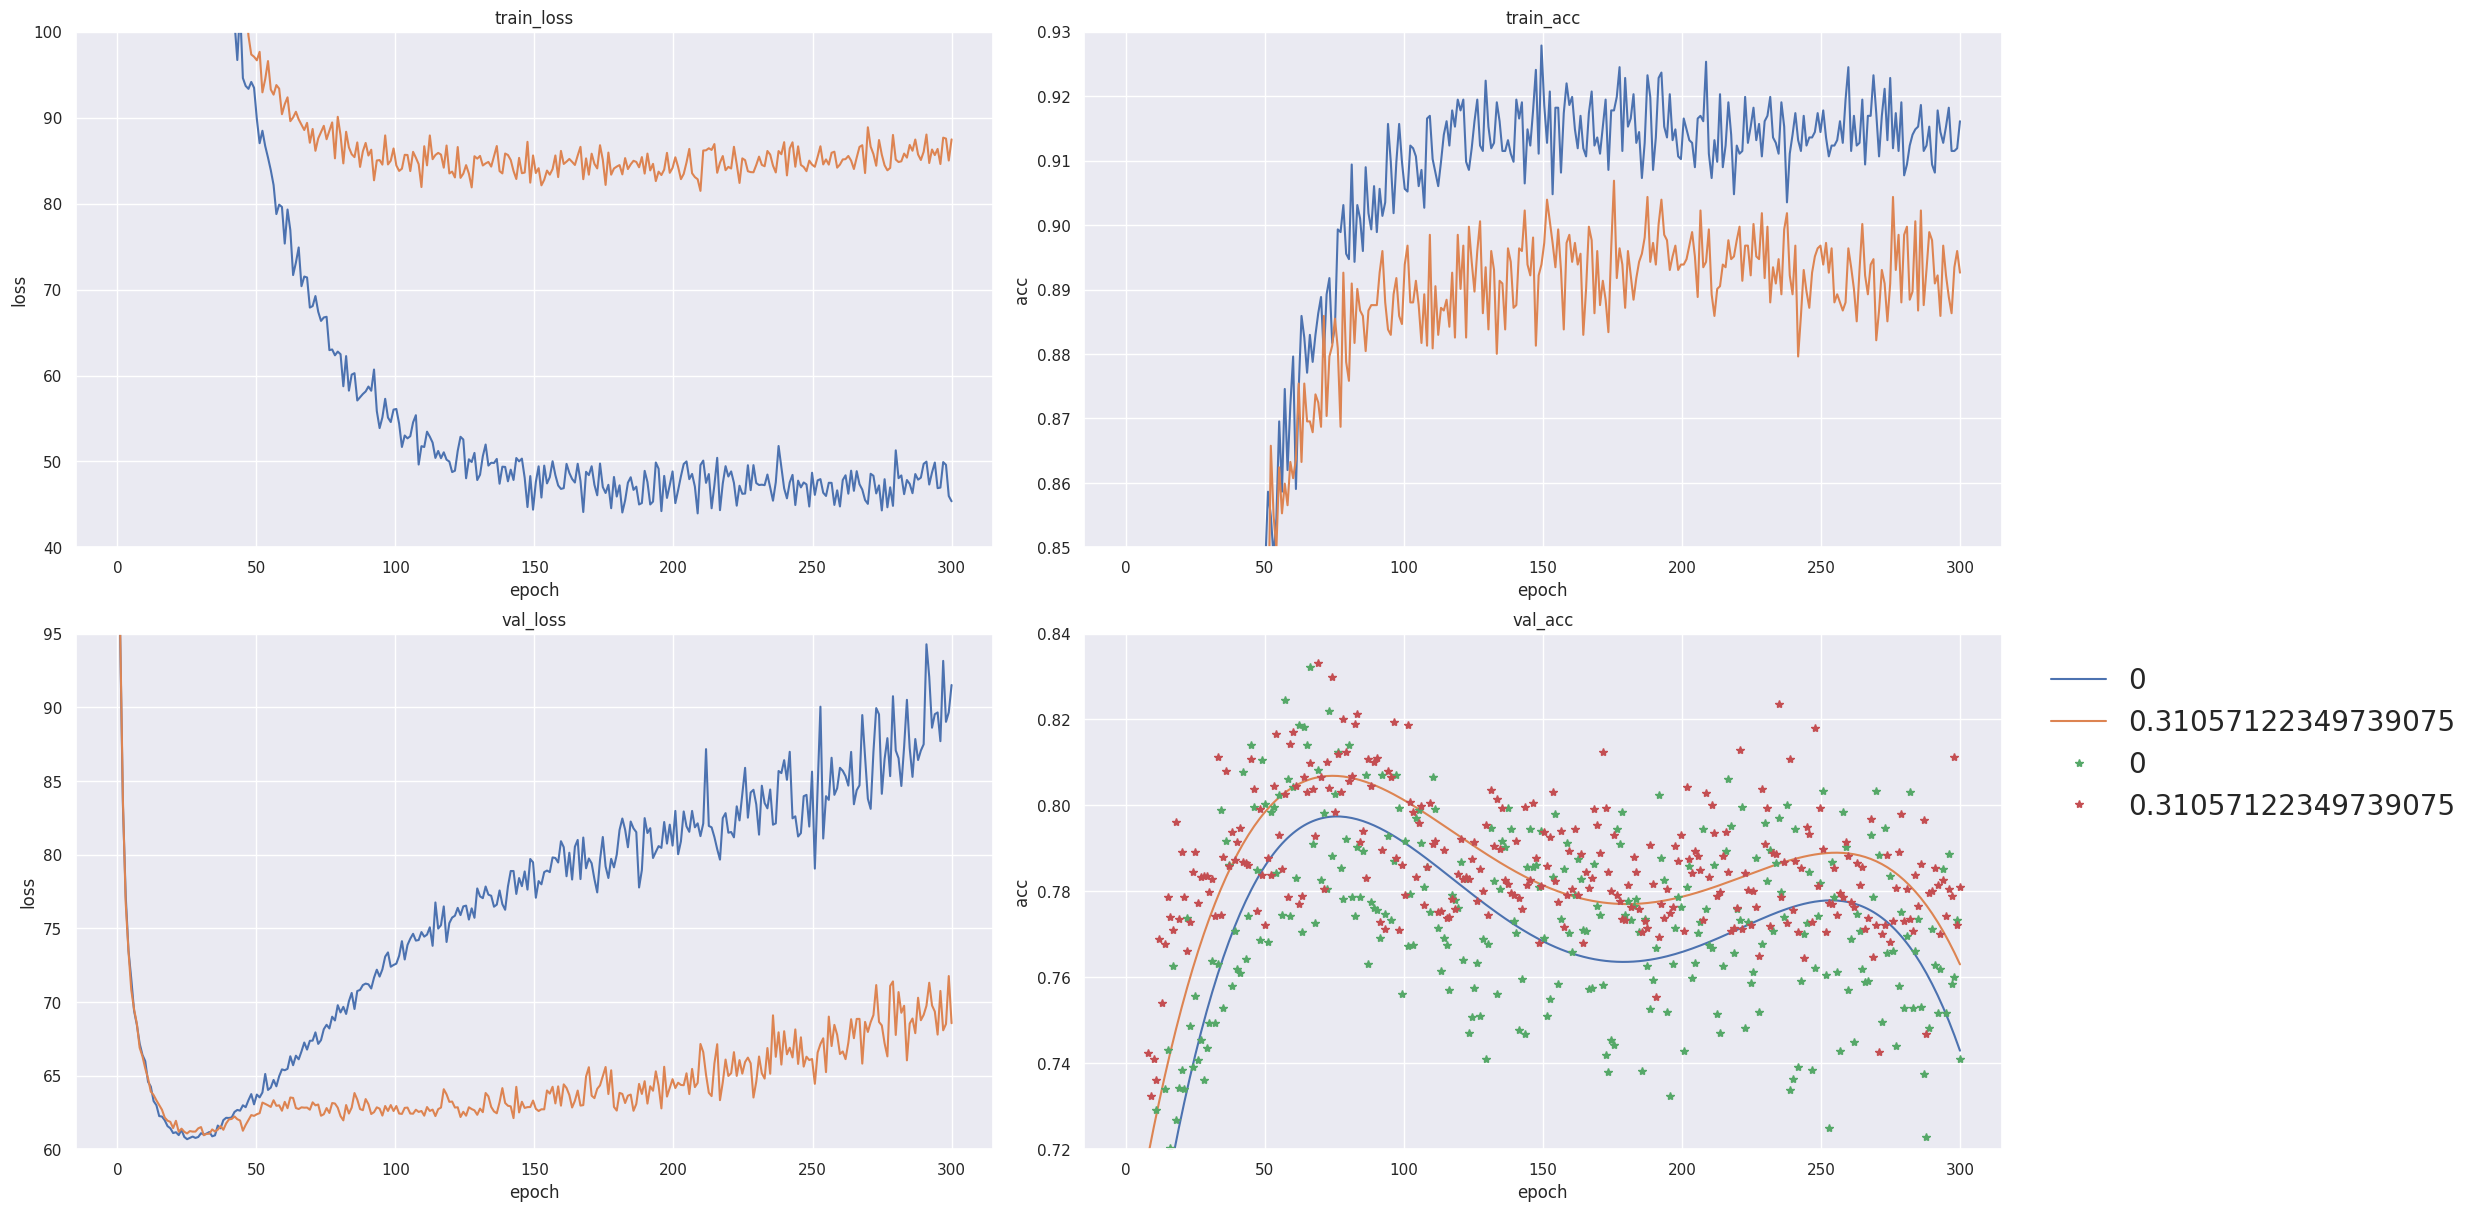
\includegraphics[width=0.75\textwidth]{figs_rev1/f8.png}
\caption{Comparative Experiment Before and After Flooding}
\label{fig:f78}
\end{figure}

We compare the two experiments without using flooding and using flooding method. The results are shown in the figure \ref{fig:f78}. The method with flooding often improves the test accuracy than the baseline method without flooding. Continuing to train the model without flooding, the loss may rise and accuracy may decline. However, according to the results which used flooding, the model has good predictive performance. The results means that flooding helps improve test accuracy in the later training. During training with flooding, test losses became lower and flatter. On the other hand, the training loss reachse a secondary decline and continues to float around the flooding threshold with stability.

\subsection{Discussion}
In this study, the data set is replaced with PlantVillage public data set and another public apple disease data set in China to conduct the pathological judgment experiment of apple leaves. In this experiment, 10 rounds of iterative experiments are conducted. The experimental results are shown in the figure below, where the apple curves represents the experimental results using the apple disease data set. The plant curves represented the experimental results using the PlantVillage public data set. 

As can be seen from the image results,\ref{fig:f9} the loss function of the training set and the test set is constantly close to 0, and the accuracy also increases with the increase of iteration rounds. The accuracy of PlantVillage public data set after applying the strategy in this paper is as high as 99\%, and the accuracy of the apple disease data set is also as high as 98.1\%, which is far higher than the 76.5\% accuracy of Zhou Minmin's apple-leaf-disease-detection-system based on transfer learning.\citep{ZhouMing} It is proved that compared with the existing strategies, the proposed strategies are universal, accurate, and less time-consuming and can better meet the needs of Chinese farmers for crop pathological judgment in today's society.
\begin{figure}
\centering
\includegraphics[width=0.75\textwidth]{figs_rev1/f9.png}
\caption{Effect experiment of mobile v3 based on flooding on different data sets}
\label{fig:f9}
\end{figure}

\section{Conclusion}
In today's society, the rise of the online QA system has brought great convenience to people's lives, but it is not widely used in agriculture. The pathological judgment of agricultural plants is an essential part of agricultural planting life. Today's crop pathological judgment mostly requires high labor costs, low detection efficiency, and poor reliability because of its dense growing environment and chaotic background. 

To solve these problems, a flood based Mobilenet v3 is proposed in this paper to identify crop leaves in fuzzy scenes. It satisfied the requirement of mobile terminal using a lightweight framework and could quickly and accurately judge crop pathological conditions through farmers' shooting pictures. The network solved most important issue about identify cucumber diseases from leaf
images in natural scenes which enable QA system for famers can be realized.

In this paper, cucumber leaf images are randomly collected from Chinese agricultural websites and labeled. A data set with complex image background is constructed, and seven kinds of cucumber leaf pathology judgments are made. Through the control variable method, the network model, the optimizer, and batch size, three rounds of experiments are compared and analyzed to achieve the optimal network model. In this paper, flooding method is used to replace an evaluation strategy of loss. The accuracy of the test set is increased by 0.5\% again, reaching the highest 83.3\%. Finally, two public data sets of Plant-Village and apple disease are selected for the experiment again. The accuracy is up to 99\% and 98.1\%, respectively, which proved the universality of the proposed strategy and its high practical value.

%\bibliographystyle{cas-model2-names}
\bibliographystyle{elsarticle-harv}
\bibliography{bibliography} 

\end{document}